\documentclass[10pt, conference, onecolumn]{IEEEtran}
\usepackage[T1]{fontenc}
\usepackage[utf8]{inputenc}
\usepackage[cmex10]{amsmath}
\usepackage{amssymb,amsfonts}
\usepackage{tikz}
\usetikzlibrary{quantikz}

\begin{document}

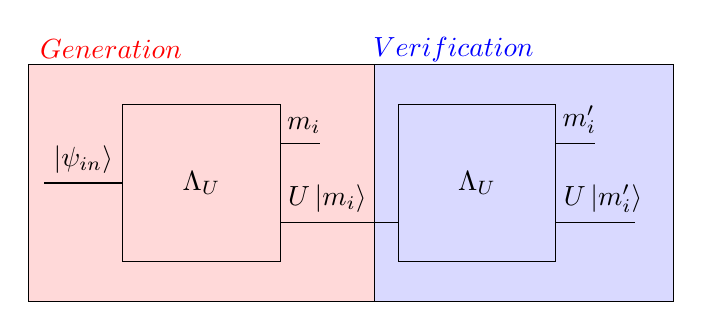
\begin{tikzpicture}
\filldraw[fill=red!15] (-1.2,2.5) rectangle (3.2,-0.5);
\filldraw[fill=blue!15] (3.2,2.5) rectangle (7,-0.5);
\draw(0,0) rectangle(2,2);
\node[red] at (-0.15,2.7) {$Generation$};
\node[blue] at (4.2,2.7) {$Verification$};
\node at (1,1) {$\Lambda_{U}$};
\draw(0,1) -- (-1,1) ;
\draw(2,1.5) -- (2.5,1.5);
\draw(2,0.5) -- (3.5,0.5);
\node[above] at (-0.5,1) {$\ket{\psi_{in}}$};
\node[above] at (2.3,1.5) {$m_{i}$};
\node[above] at (2.6,0.5) {$U\ket{m_{i}}$};

\draw(3.5,0) rectangle(5.5,2);
\node at (4.5,1) {$\Lambda_{U}$};
\draw(5.5,1.5) -- (6,1.5);
\node[above] at (5.8,1.5) {$m'_{i}$};
\draw(5.5,0.5) -- (6.5,0.5);
\node[above] at (6.1,0.5) {$U \ket{m'_{i}}$};
\end{tikzpicture}

\end{document}